% This LaTeX was auto-generated from MATLAB code.
% To make changes, update the MATLAB code and export to LaTeX again.

\documentclass{article}

\usepackage[utf8]{inputenc}
\usepackage[T1]{fontenc}
\usepackage{lmodern}
\usepackage{graphicx}
\usepackage{color}
\usepackage{listings}
\usepackage{hyperref}
\usepackage{amsmath}
\usepackage{amsfonts}
\usepackage{epstopdf}
\usepackage[table]{xcolor}
\usepackage{matlab}

\sloppy
\epstopdfsetup{outdir=./}
\graphicspath{ {./AnimatedPlots_images/} }

\begin{document}

\matlabtitle{Example: Animated Plots}

\begin{par}
\begin{flushleft}
Having animated plots would be cool. Let's try to figure out how to export them as video files or animated GIFs or something.
\end{flushleft}
\end{par}

\matlabheading{Plots using for loops}

\begin{par}
\begin{flushleft}
Here's an example of animated plots that you get when you plot stuff in a loop in a Live Script.
\end{flushleft}
\end{par}

\begin{matlabcode}
ax = axes;
axis(ax, [0, 2*pi, -1, 1])
hold(ax, "on")

for i = linspace(0, 2*pi)
    scatter(ax, i, cos(i), 'b')
    drawnow
    pause(0.025)
end
\end{matlabcode}
\begin{center}
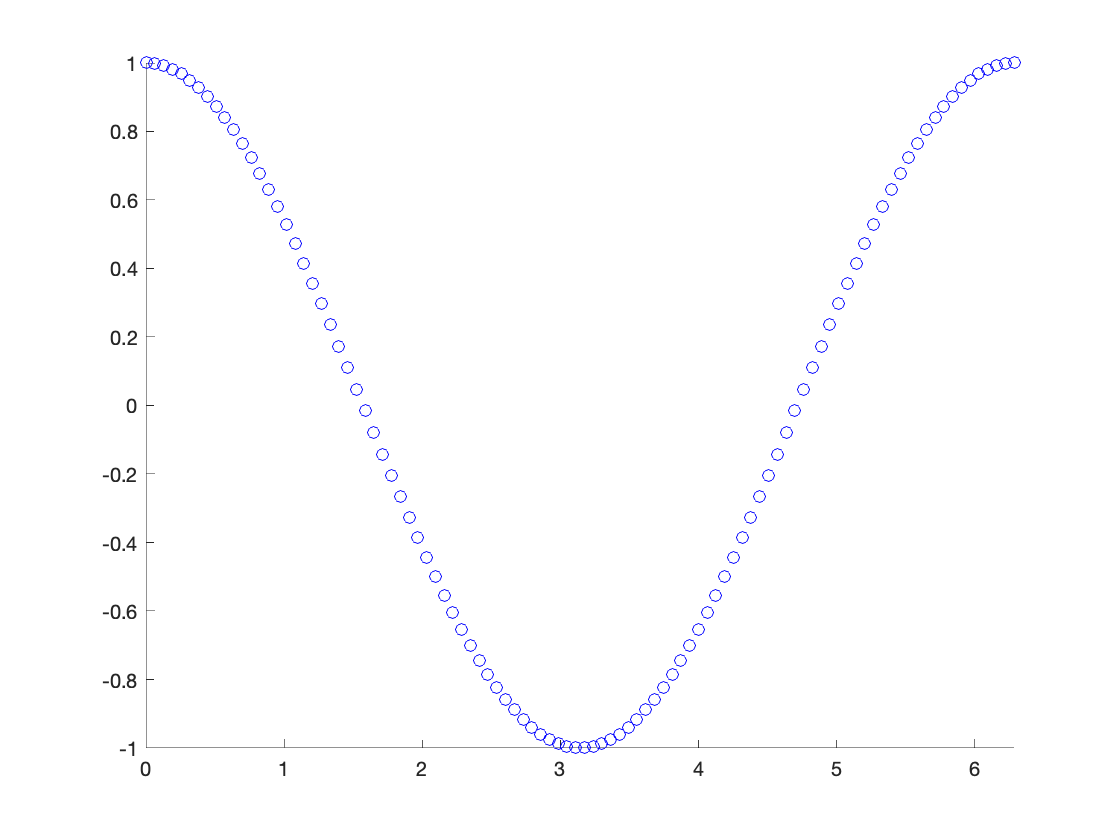
\includegraphics[width=\maxwidth{56.196688409433015em}]{figure_0.png}
\end{center}

\begin{par}
\begin{flushleft}
When you run the Live Script, it only does one pass through the sequence. How should we handle that?
\end{flushleft}
\end{par}

\matlabheading{Plots using movie}

\begin{par}
\begin{flushleft}
Maybe you can also do animated plots using the \texttt{movie} function.
\end{flushleft}
\end{par}

\begin{par}
\begin{flushleft}
First, you have to enable it in the editor:
\end{flushleft}
\end{par}

\begin{matlabcode}
if verLessThan('matlab', '9.10.0')
    mlSettings = settings;
    mlSettings.matlab.editor.AllowFigureAnimation.TemporaryValue = 1;
end
\end{matlabcode}

\begin{par}
\begin{flushleft}
(This is probably not safe to do in widely-used Live Scripts. An \texttt{onCleanup} and a \texttt{clear} could somewhat take care of this.)
\end{flushleft}
\end{par}

\begin{par}
\begin{flushleft}
Record the movie:
\end{flushleft}
\end{par}

\begin{matlabcode}
% Code taken from Matlab's `doc movie`
figure
Z = peaks;
surf(Z)
axis tight manual
\end{matlabcode}
\begin{center}
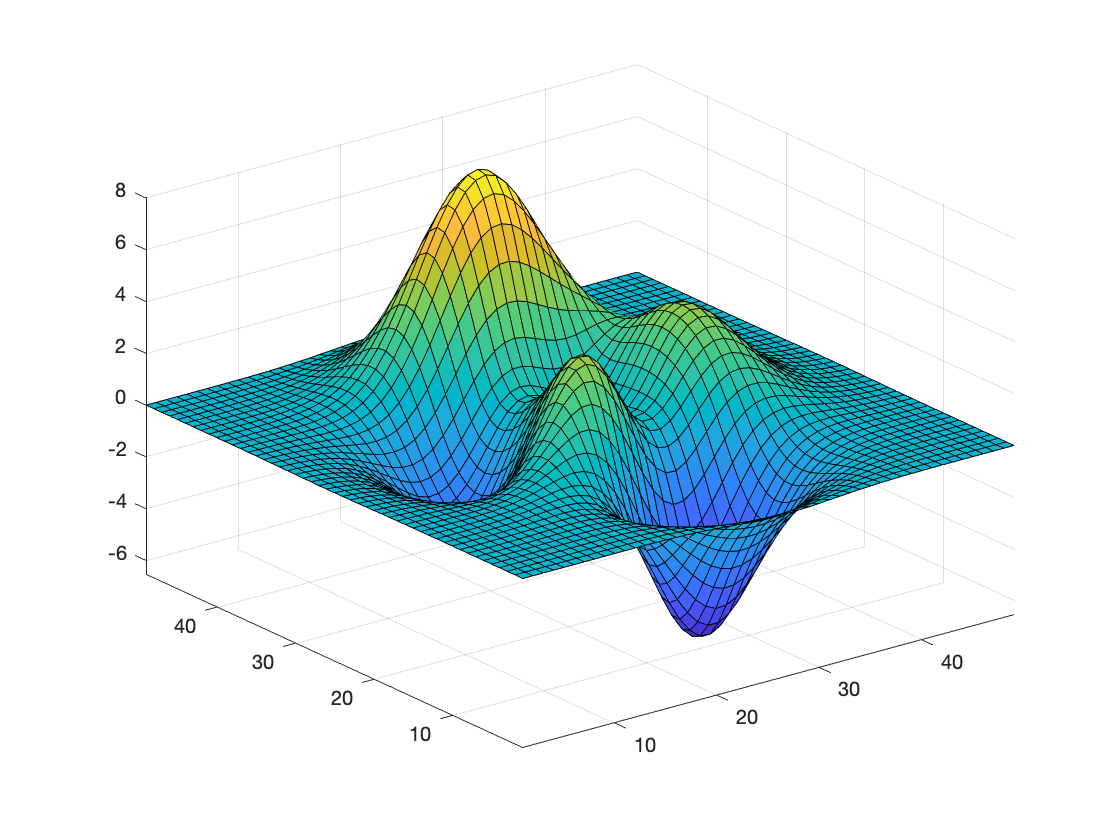
\includegraphics[width=\maxwidth{56.196688409433015em}]{figure_1.png}
\end{center}
\begin{matlabcode}
ax = gca;
ax.NextPlot = 'replaceChildren';

loops = 40;
F(loops) = struct('cdata',[],'colormap',[]);
for i = 1:loops
    X = sin(i*pi/10)*Z;
    surf(X,Z);
    drawnow
    F(i) = getframe;
end
\end{matlabcode}

\begin{par}
\begin{flushleft}
Then play it back:
\end{flushleft}
\end{par}

\begin{matlabcode}
movie(F,2);
\end{matlabcode}
\begin{center}
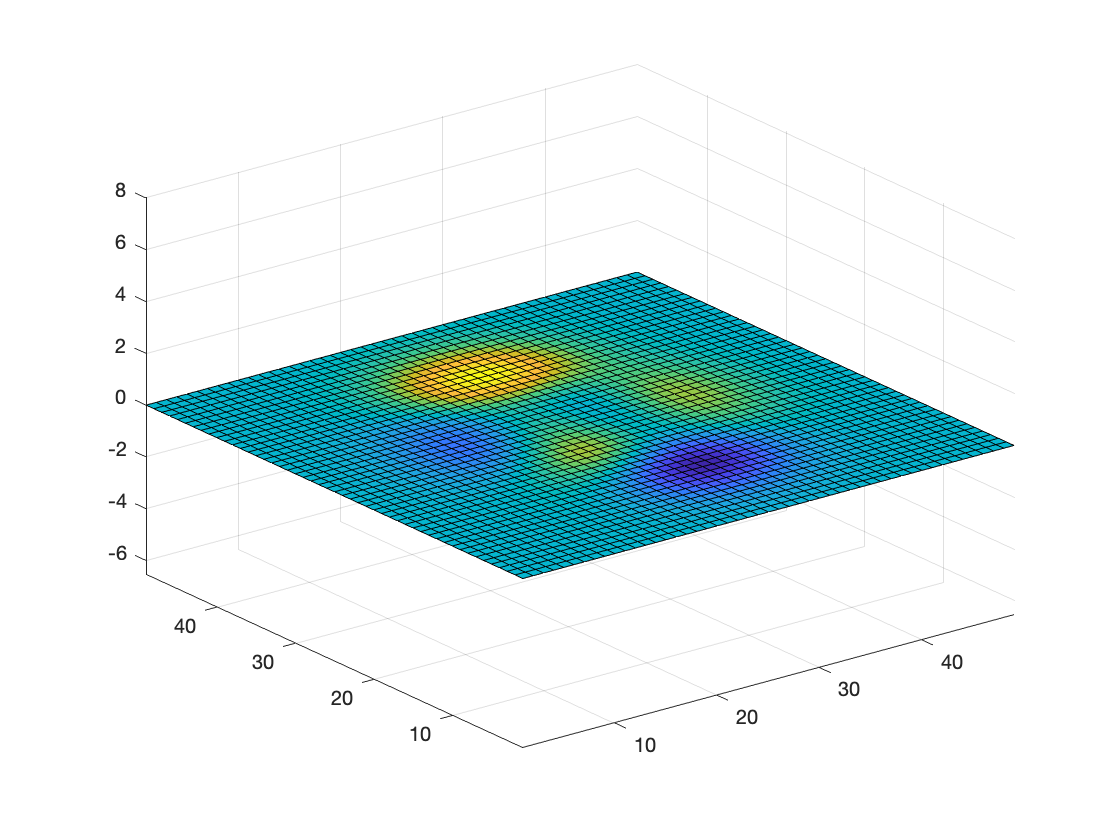
\includegraphics[width=\maxwidth{56.196688409433015em}]{figure_2.png}
\end{center}

\begin{par}
\begin{flushleft}
Does that work?
\end{flushleft}
\end{par}

\begin{par}
\begin{flushleft}
Hmm. Doesn't look like it.
\end{flushleft}
\end{par}

\matlabheading{New R2021a Live Script movie support}

\begin{par}
\begin{flushleft}
R2021a has better support for this: \href{https://blogs.mathworks.com/pick/2021/03/26/animation-playback-controls-in-live-scripts-r2021a/.}{https://blogs.mathworks.com/pick/2021/03/26/animation-playback-controls-in-live-scripts-r2021a/.} I can't get that to work yet, though.
\end{flushleft}
\end{par}

\begin{par}
\begin{flushleft}
Note: R2021 release notes say: "Animation playback controls are not supported for animations generated by the \texttt{movie} function."
\end{flushleft}
\end{par}

\end{document}
